\section{Methods}

There were two main parts of 2to3D we needed to implement: the user interface and the geometric constraint solver. For each of these tasks, we employed a different library, with lots of JavaScript code glueing them together.

\subsection*{User Interface with React.js}

React.js is an innovative JavaScript library that allows the programmer to specify different parts of the interface as {\it components}. Each component manages its own state and has its own render function. Whenever a component's state is changed, React automatically re-renders it, effectively abstracting the render loop from the programmer. In this way, a typical React App need only deal with event handling by manipulating state.

2to3D consists of one main DrawArea component, whose state contains all the primitive shape objects, along with the constraints on these objects, so that when the user draws a new shape or modifies an existing one, the interface is re-rendered.

%The state of each object consists of where it is located in the drawing region and whether or not the shape is selected. Furthermore, each shape maintains its own render method, which is based on the aforementioned aspects of state.

Currently, we have the following shape primitives:

\begin{itemize}
\item {\bf Freehand Curves}
\item {\bf Lines}
\item {\bf Bezier Curves}
\end{itemize}

Freehand curves are simply SVG paths, but within Line and Bezier objects are points whose values can be manipulated, both by the user and the constraint solver. We discuss this in more detail in the next section, but with these shape primitives we created the following drawing tools:

\begin{itemize}
\item {\bf Freehand:} Simply draws a freehand curve following the cursor.
\item {\bf Polyline:} Creates lines where adjacent endpoints are constrained to be coincident, optionally allowing the user to close the polyline where it started, creating a polygon.
\item {\bf Bezier:} Creates bezier curves whose adjacent endpoints are constrainted to be coincident and adjacent control points are constrained to be collinear with the endpoint between them.
\item {\bf Rectangle:} Creates four lines in a rectangle where the top and bottom lines are constrained to be horizontal and the left and right lines are constrained to be vertical.
\end{itemize}

\subsection*{Geometric Constraints with Cassowary.js}

In order to design physical objects for laser cutting, we needed our program to implement geometric constraints. For example, we would like to be able to specify two lines as parallel, or a line have fixed length. All of the constraints we wanted to implement can be represented as systems of equations. For example, consider Figure \ref{fig:constraints} below. We constrain point $a$ to always lie on the circle of radius 1, we fix the line with endpoints $a$ and $b$ to have length $\sqrt{2}$ using the distance equation, and we set the line with endpoints $b$ and $c$ to lie on the $x$-axis and have length 1.

\begin{figure}[H]
  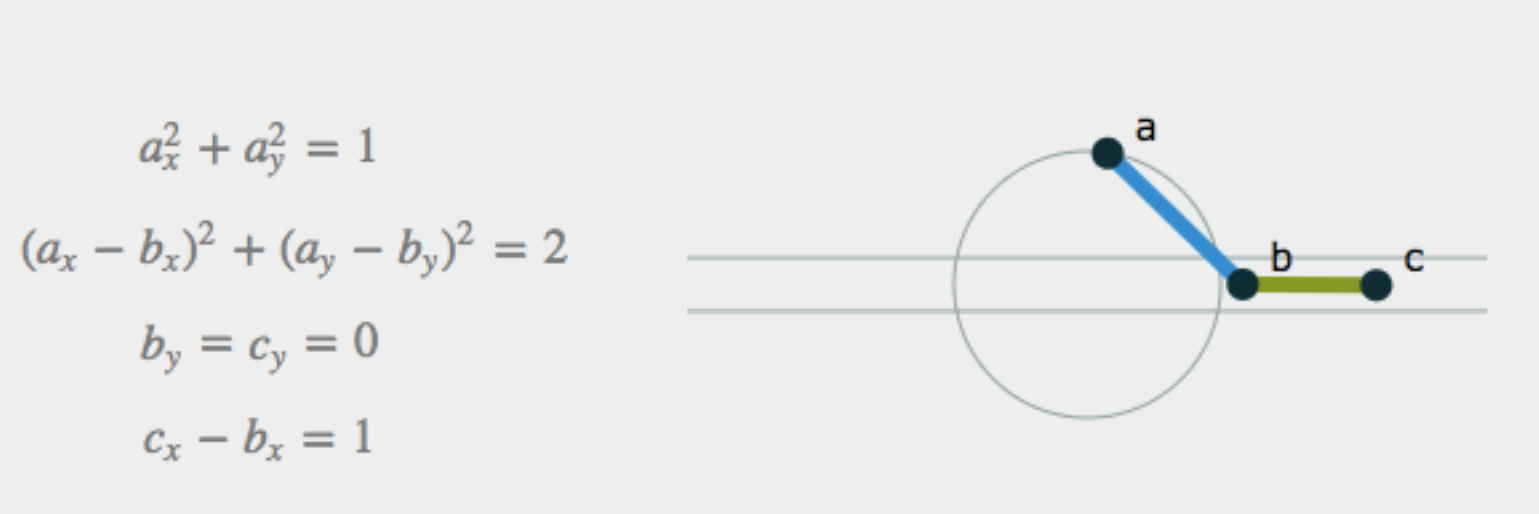
\includegraphics[width=\linewidth]{constraints.jpg}
  \caption{Parametric constraints represented as equations and inequalities; adapted from Ref. \cite{keeter}. }
  \label{fig:constraints}
\end{figure}

The interface allows the user to freely click-and-drag points around the canvas, which creates the problem of satisfying all the constraints in real-time. To tackle this problem, we found Cassowary.js \cite{cassowary}, a JavaScript library that implements a version of the simplex algorithm, which was created to solve {\it linear programming} problems.  A linear program consists of $n$ variables on which we have a linear objective function and a set of linear constraints. For example, the following is a linear program on $n=4$ variables.
\[\text{Minimize } C = x_1 + 3x_2 - 2x_4 \text{ subject to: }\]
\[x_1 + x_2 \geq 4,\]
\[x_3 - 4x_4 + x_2 = 42, \text{ and}\]
\[4x_1 + x_3 - x_2 \leq 2.\]

Therefore, we can formulate our geometric constraints as a linear program where each $x$ and $y$ value of every point in every shape is a variable and each geometric constraint is transformed into (possibly multiple) linear constraints. In addition to solving simple linear programs, Cassowary.js also allows us to specify non-required constraints of varying {\it strength}. For example, we can specify that we would like a particular point to stay where it is unless absolutely necessary. Because of this, we do not need to explicitly define an objective function for our linear program.

Some geometric constraints are easily transformed into linear (in)equalities, but others are not. For example, to constrain a line to be horizontal is easy, as we simply specify that the $x$ coordinates of its endpoints must be equal, but constraining a line to be a fixed length is much more difficult. Our solution was to cleverly reform and approximate many geometric constraints using more than one linear equation or inequality.

Below are the geometric constraints we implemented, along with a description of how they were implemented. 

\begin{itemize}
\item {\bf Fixed:} Constrains a point to stay in the same location. Implemented by setting the $x$- and $y$-coordinates to be constants.
\item {\bf Coincident:} Constrains two points to lie in the same location. Implemented by setting the x-coordinates to be equal and the y-coordinates to be equal.
\item {\bf Horizontal:} Constrains a line to be horizontal. Implemented by setting the x-coordinates of the two endpoints to be equal.
\item {\bf Vertical:} Constrains a line to be vertical. Implemented by setting the y-coordinates of the two endpoints to be equal.
\item {\bf Parallel:} Constrains two lines to be parallel. This constraint is more difficult to implement, as there is no way to represent it with linear equations. However, we can implement a fixed-slope constraint using linear equations by fixing the ratio between the difference of the $x$- and $y$- coordinates. So, when this constraint is initially set, we constrain both lines to have a fixed slope, and whenever an endpoint is moved, we programmatically update the slope of the constraint.
\item {\bf Perpendicular:} Constrains two lines to be perpendicular. This constraint is implemented exactly the same as the parallel constraint, except for setting both lines to have the same slope, one is set to have the negative reciprocal slope of the other and is updated programmatically in a similar way.
\item {\bf Length:} Constrains a line to be a fixed length. This was the most difficult constraint to implement, as the distance equation is very nonlinear, so instead we must approximate it with many linear inequalities. The {\it Manhattan distance} is defined as the sum of the absolute differences between the $x$- and $y$-coordinates of two points. So, we can estimate a Euclidean distance constraint with multiple Manhattan distance constraints in the following way. If we constrain a point to be within a fixed Manhattan distance of another point, the it will lie within a diamond centered at that point. Then, using linear equations, we can transform our coordinate system by a fixed angle and set another Manhattan distance distance constraint. This constraint will have the diamond rotated by that fixed angle. Enough of these constraints will approximate a circle. However, this only constrains two points to be {\it within} a fixed distance, so we must create minimum Manhattan distance constraints in a similar way. All of these together allows us to constrain the two endpoints of a line to a fixed distance from each other. This process is illustrated in Figures \ref{dist1} through \ref{dist3}.
\end{itemize}

\begin{figure}[H]
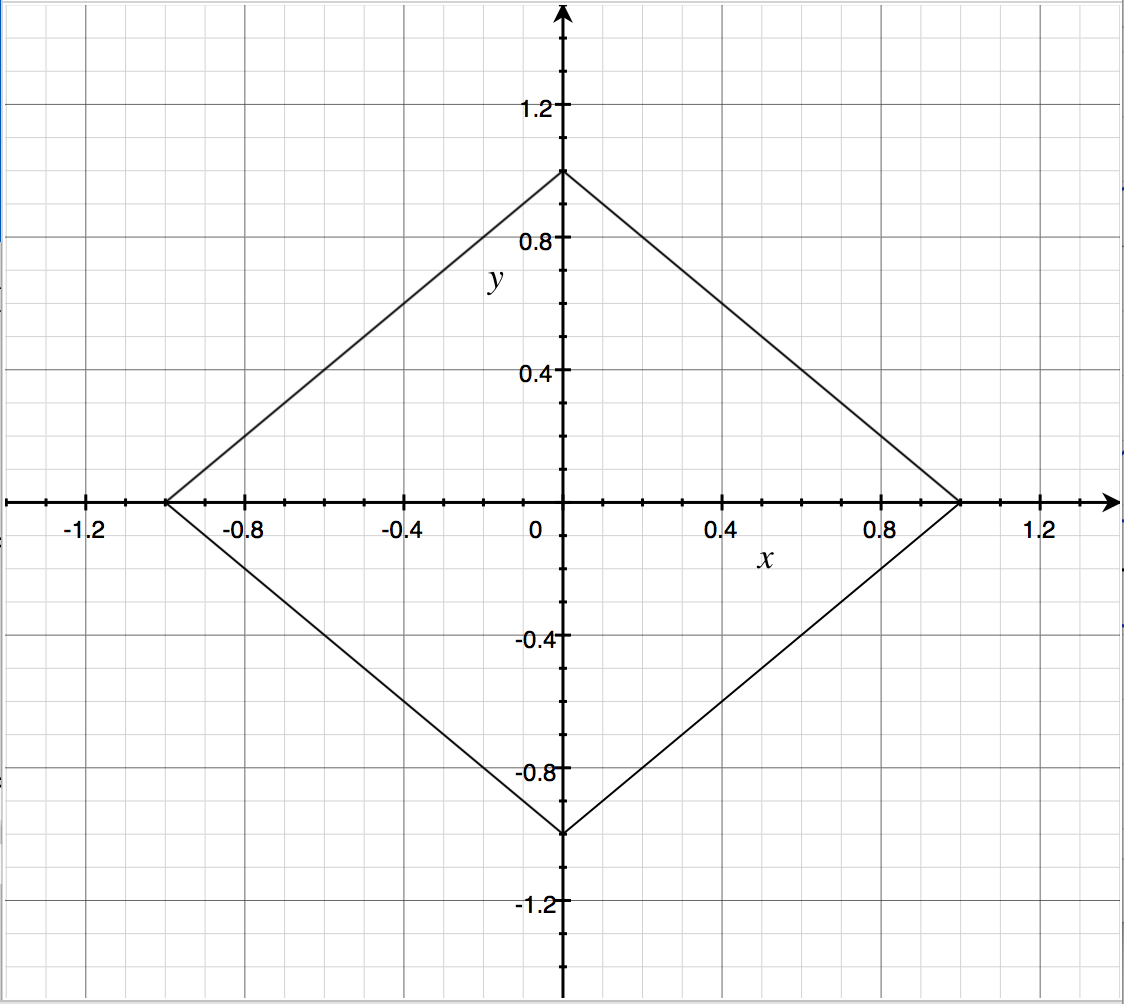
\includegraphics[width=\linewidth]{dist1.png}
\caption{The region constrained by $|x| + |y| \leq 1$.}
\label{dist1}
\end{figure}

\begin{figure}[H]
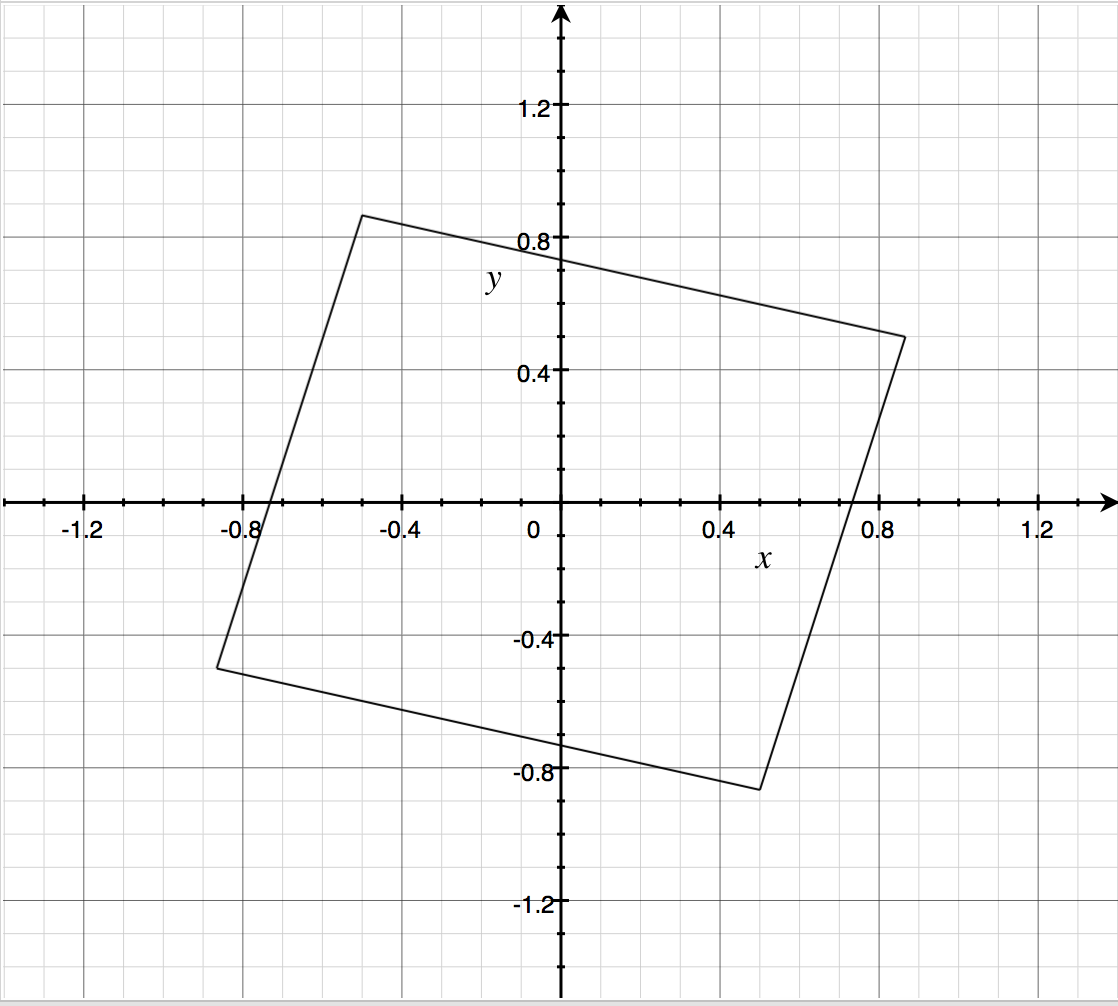
\includegraphics[width=\linewidth]{dist2.png}
\caption{The region constrained by $|x'| + |y'| \leq 1$ where $x'$ and $y'$ are the coordinates of the point in the coordinate system rotated by 30$^\circ$.}
\label{dist2}
\end{figure}

\begin{figure}[H] 
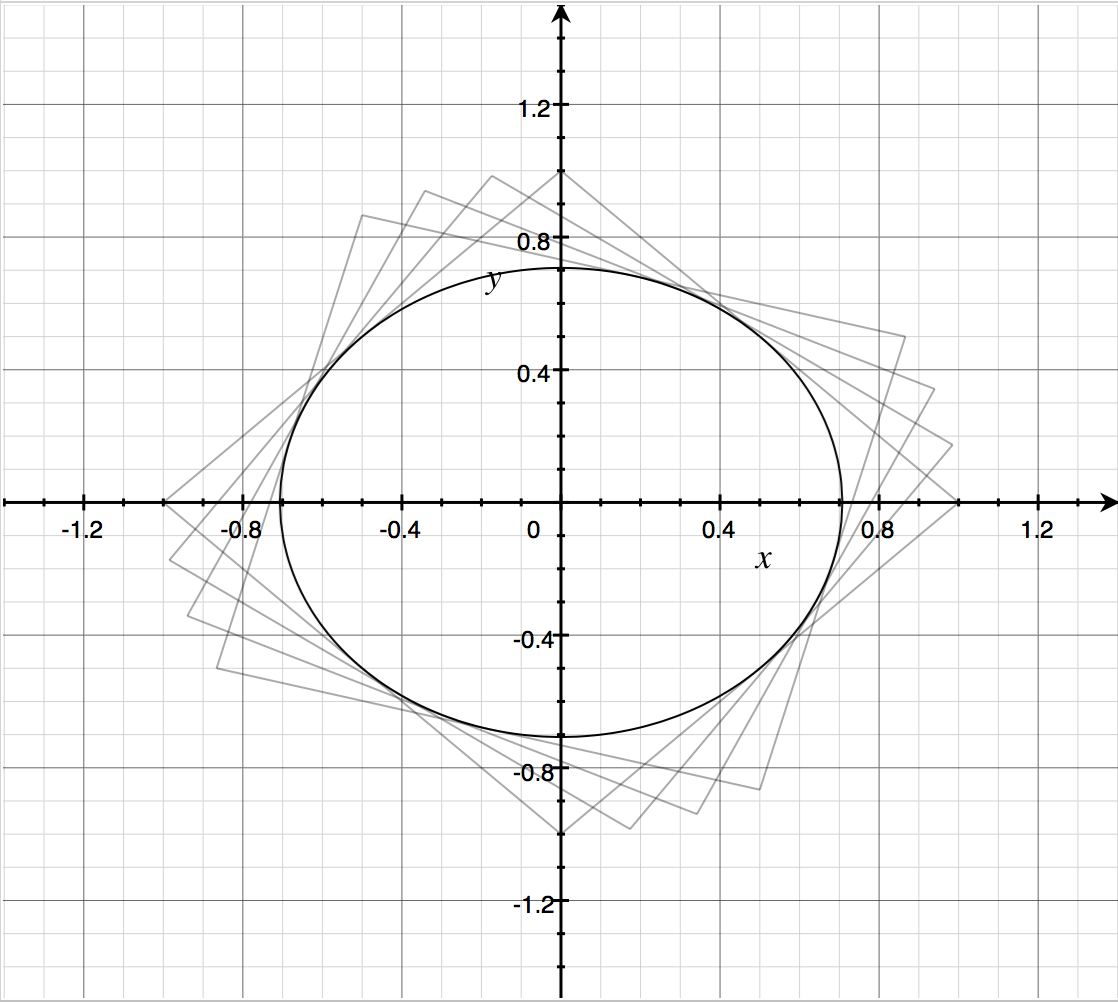
\includegraphics[width=\linewidth]{dist3.png}
\caption{With enough of these regions, we approximate the circle of radius $\frac{\sqrt{2}}{2}$ about the origin.}
\label{dist3}
\end{figure}

The full implementation can be found at TODO LINK.





\begin{comment}
This section should include the following:
\begin{itemize}
		
\item	A description of the methods you are using (which itself could have
	sub-sections). If you have created a new application, you should describe
	which tools you have used to do so and the steps of your implementation. You
	should also briefly describe each of the tools you used (e.g. Ruby on Rails,
	MongoDB, D3, etc.). If you have proposed a new algorithm to solve a problem,
	you should provide the details of your algorithm along with pseudocode. If
	your algorithm is quite complex, you should describe its running time.  

\item Description of any data you used and explanation of why you chose this
	particular data (possibly organized into sub-sections).

\item Link to a GitHub, BitBucket or other repository if relevant.

\end{itemize}
\end{comment}